% !TEX encoding = UTF-8 Unicode
\documentclass[a4paper]{article}

\usepackage{color}
\usepackage{url}
\usepackage{xurl}
\usepackage[T2A]{fontenc} % enable Cyrillic fonts
\usepackage[utf8]{inputenc} % make weird characters work
\usepackage{graphicx}

\usepackage[english,serbian]{babel}
%\usepackage[english,serbianc]{babel} %ukljuciti babel sa ovim opcijama, umesto gornjim, ukoliko se koristi cirilica

\usepackage[unicode]{hyperref}
\hypersetup{colorlinks,citecolor=green,filecolor=green,linkcolor=blue,urlcolor=blue}

\usepackage{listings}

%\newtheorem{primer}{Пример}[section] %ćirilični primer
\newtheorem{primer}{Primer}[section]

\definecolor{mygreen}{rgb}{0,0.6,0}
\definecolor{mygray}{rgb}{0.5,0.5,0.5}
\definecolor{mymauve}{rgb}{0.58,0,0.82}

\lstset{ 
  backgroundcolor=\color{white},   % choose the background color; you must add \usepackage{color} or \usepackage{xcolor}; should come as last argument
  basicstyle=\scriptsize\ttfamily,        % the size of the fonts that are used for the code
  breakatwhitespace=false,         % sets if automatic breaks should only happen at whitespace
  breaklines=true,                 % sets automatic line breaking
  captionpos=b,                    % sets the caption-position to bottom
  commentstyle=\color{mygreen},    % comment style
  deletekeywords={...},            % if you want to delete keywords from the given language
  escapeinside={\%*}{*)},          % if you want to add LaTeX within your code
  extendedchars=true,              % lets you use non-ASCII characters; for 8-bits encodings only, does not work with UTF-8
  firstnumber=1000,                % start line enumeration with line 1000
  frame=single,	                   % adds a frame around the code
  keepspaces=true,                 % keeps spaces in text, useful for keeping indentation of code (possibly needs columns=flexible)
  keywordstyle=\color{blue},       % keyword style
  language=Python,                 % the language of the code
  morekeywords={*,...},            % if you want to add more keywords to the set
  numbers=left,                    % where to put the line-numbers; possible values are (none, left, right)
  numbersep=5pt,                   % how far the line-numbers are from the code
  numberstyle=\tiny\color{mygray}, % the style that is used for the line-numbers
  rulecolor=\color{black},         % if not set, the frame-color may be changed on line-breaks within not-black text (e.g. comments (green here))
  showspaces=false,                % show spaces everywhere adding particular underscores; it overrides 'showstringspaces'
  showstringspaces=false,          % underline spaces within strings only
  showtabs=false,                  % show tabs within strings adding particular underscores
  stepnumber=2,                    % the step between two line-numbers. If it's 1, each line will be numbered
  stringstyle=\color{mymauve},     % string literal style
  tabsize=2,	                   % sets default tabsize to 2 spaces
  title=\lstname                   % show the filename of files included with \lstinputlisting; also try caption instead of title
}


\usepackage{csquotes}
\MakeOuterQuote{"}

\begin{document}

\title{Doktorske studije informatike u Srbiji\\ \small{Seminarski rad u okviru kursa\\Metodologija stručnog i naučnog rada\\ Matematički fakultet}}

\author{Ivan Pop-Jovanov, Tatjana Kunić, Viktor Novaković, Pavle Cvejović\\ mi18085@alas.matf.bg.ac.rs, mi17139@alas.matf.bg.ac.rs, \\mi18092@alas.matf.bg.ac.rs, mi18024@alas.matf.bg.ac.rs}

%\date{9.~april 2015.}

\maketitle

\abstract{
U ovom radu predstvljamo na jednom mestu sve informacije koje bi bile korisne nekome ko se interesuje za doktorske akadmske studije informatike u Srbiji. Odgovaramo na pitanja šta su doktorske studije, kako ih upisati i koje mogućnosti nam otvaraju u Srbiji.}

\tableofcontents

\newpage

\section{Uvod}
\label{sec:uvod}

Studenti informatike na poslednjim godinama svojih osnovnih ili master studija često se sreću sa pitanjem "Šta dalje?" Da li nastaviti svoje usavršavanje na fakultetu, ili prvom mogućom prilikom ući u industriju? Da li doktorske studije mogu da pomognu pri kasnijim uspesima u industriji, ili su samo korisne individuama koje žele da se bave naukom? Ovaj rad ima za cilj da na jednom mestu sakupi informacije na temu i da prikaže pogled odozgo na različite aspekte doktorskih studija informatike u Srbiji.

U sekciji dva govorimo uopšteno o doktorskim studijama, šta su to doktorske studije i kako izgleda njihova struktura i organizacija. Treća sekcija ulazi u detalje procesa i zahteva za upis na doktorske studije različitih fakulteta u Srbiji. U četvrtoj sekciji se osvrćemo na izgled samih studija na fakultetima u Srbiji. Za kraj, u petoj sekciji razmatramo veze između doktorskih studija informatike i IT industrije u Srbiji.

\section{Uopšteno o doktorskim studijama}
\label{sec:uopsteno}

U ovom poglavlju ćemo ispričati šta su to doktroske studije, kako su organizovane i koja je njihova struktura kao i koliko je njihovo vreme trajanja propisano planom i programom fakulteta i koliko vremena zaista treba studentima da bi ih zavšili. Relevantne informacije smo uzeli sa više od 10 fakulteta u kojima postoji smer (ili odsek) za infromatiku, neki od kojih su Elektrotehnički fakultet, Fakultet organizacionih nauka, Mašinski fakultet u Beogradu, Fakultet za informacione tehnologije i inžinjerstvo, Prirodno-matematički fakultet u Novom Sadu i Kragujevcu\cite{fondoktorske, matfbgdoktorske, matfnsdoktorske, etfdoktorske}...

\subsection{Šta su to doktorske studije?}

Doktorske studije informatike su jedinstveni istraživački stepen definisan inovativnom primenom i pronalaskom računarskih metoda za unapređenje postojećih ili novostvorenih oblasti istraživanja. Istraživanje i obrazovanje u informatici imaju snažan interdisciplinarni fokus koji spaja osnove informacija i računarstva sa oblastima primene.



\subsection{Organizacija i struktura studija}

Doktorske studije su na većini gorepomenutih fakulteta organizovane tako da omoguće aktivan naučni razvoj kandidata i koncipirane su tako da pružaju slobodan izbor svih predmeta u dogovoru sa predmetnim profesorima koji odlučuju na koji način će se polagati ti predmeti, bilo preko usmenih i pismenih provera ili preko projekata. 

Svakom studentu se takođe dodeljuje \emph{savetnik} (tutor) koga student bira pri početku studija čija je uloga da pomogne studentu pri koncipiranju stručne i naučne specifičnosti u realizaciji studija. 

Pre izrade ili odbrane završnog rada, odnosno doktorske disertacije, neki fakulteti zahtevaju da student ima barem jedan objavljen i prihvaćen naučni rad za štampu u časopisu sa \emph{SCI liste}. 

Konačno, na kraju studija, student izrađuje \emph{doktorsku disertaciju} koja predstavlja samostalni naučni rad studenta i nakon što zadovolji uslove neophodne za odbranu disertacije i uspešno je odbrani student stiče zvanje \emph{doktor nauka} iz relevantne naučne oblasti.

\subsection{Vreme trajanja doktorskih studija}

Što se tiče trajanja doktorskih studija po planu i programu fakulteta, na svim fakultetima pomenutim na početku ovog poglavlja je situacija ista, doktorske studije traju 3 godine i nose 180 ESPB bodova kao i na našem, Matematičkom fakultetu u Beogradu\cite{matfbgdoktorske}.


Sa druge strane, istraživali smo koliko je studentima (tj. kandidatima) zaista trebalo vremena da završe doktorske studije, tako što smo te podatke preuzeli od skoro 40 ljudi sa \emph{LinkedIn}-a koji su završili doktorske studije na temu informatike i računarstva u Srbiji na prethodno pomenutim fakultetima i po slici \ref{fig:statistics-bar} vidimo da većina studenata ne završi doktorske studije za vreme propisano planom i programom fakulteta već je realnije vreme trajanja doktorskih studija 4 ili 5 godina. 

\begin{figure}[h!]
\begin{center}
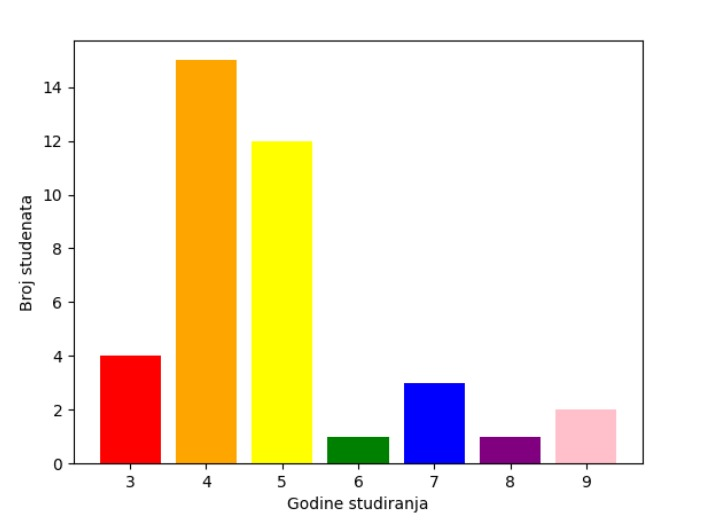
\includegraphics[scale=0.4]{DuzinaStudija.png}
\end{center}
\caption{Realno vreme trajanja doktorskih studija}
\label{fig:statistics-bar}
\end{figure}

\section{Uslovi upisa}
\label{sec:uslovi}

Da bi lice moglo da konkuriše na doktorske akademske studije informatike u Srbiji, mora da zadovolji određene uslove koje zadaje fakultet na kom se održavaju. Pravilnik o doktorskim studijama koje organizuje i izvodi Univerzitet u Beogradu\cite{pravilnik}, u članu 6, navodi da se znanja i sposobnosti potrebne za upis, kao i način provere, objavljuju u konkursu. Univerzitet u Beogradu definiše opšte uslove konkursa, ali svaki fakultet objavljuje svoj posebni konkurs. 

\subsection{Opšti uslovi Univerziteta u Beogradu}

Dokument "Opšti uslovi konkursa Univerziteta u Beogradu"\cite{konkursBeograd} navodi sledeće uslove (delovi narednog teksta su preuzeti direktno iz Konkursa, sa malim stilskim izmenama, a za detaljnije informacije pogledati originalni dokument). 

Na doktorske studije može konkurisati lice koje ima završene osnovne akademske i master akademske studije, ili integrisane studije sa najmanje 300 ESPB bodova. Takođe, može konkurisati i lice koje ima završene najmanje četvorogodišnje studije po propisima koji su važili do stupanja na snagu \emph{Zakona o visokom obrazovanju} ("Sl. glasnik RS", br. 76/2005, 100/2007 - autentično tumačenje, 97/2008, 44/2010, 93/2012, 89/2013, 99/2014, 45/2015 - autentično tumačenje, 68/2015 i 87/2016). 

Lice mora imati opštu prosečnu ocenu od najmanje 8,00 na dosadašnjim studijama. Postoji i mogućnost konkurisanja za lica koji imaju prosečnu ocenu manju od 8,00, ako imaju ostvarene naučne radove objavljene u časopisima sa liste resornog ministarstva pre upisa na doktorske studije, u skladu sa opštim aktima fakulteta, odnosno Univerziteta. Potrebno je da lice zna jedan svetski jezik, dok određeni fakulteti traže specifično engleski, i za upis u 2022/2023 godini, potrebno je da je prethodne studije završila najkasnije 14. oktobra 2022. godine. 

Upis na doktorske studije je takođe omogućeno i licima koje imaju akademski stepen magistra nauka u istoj ili srodnoj naučnoj oblasti, ako ispunjavaju uslove koji su konkursom predviđeni za upis. Na lični zahtev može im se priznati i deo sadržaja nastavnog plana magistarskih studija, ali moraju da ostvare najmanje 90 ESPB na studijskom programu doktorskih studija koji su upisali, koji se odnose na istraživanje, izradu i odbranu doktorske disertacije. 

Dodatna opcija postoji i za lica koja su započela doktorse studije u istoj ili srodnoj naučnoj oblasti na drugoj visokoškolskoj ustanovi, pod uslovima utvrđenim studijskim programom, na način i po postupku opštim aktima Univerziteta i fakulteta. Mora ispunjavati uslove za upis i može se upisati samo kao samofinansirajući student. Ovako upisani studenti se ne ubrajaju u odobreni broj studenata za određeni studijski program. 

\subsection{Merila za utvrđivanje redosleda kandidata}

Isti dokument\cite{konkursBeograd} definiše i preporuke za rangiranje kandidata za 2022/23 godinu. Parametri koji se koriste za utvrđivanje redosleda su opšta prosečna ocena i dužina studiranja na dosadašnjim studijama, kao i ostvareni naulni rezultati. Moguće je u proces kvalifikacije uračunati i razgovor (intervju) sa kandidatom, a dozvoljeno je i da fakultet uvede dodatne kriterijume. 

\subsection{Matematički fakultet}

Malo detaljnije ćemo opisati posebne uslove konkursa Matematičkog fakulteta\cite{konkursMATF}, a za ostale fakultete ćemo samo ukratko opisati razlike. 

Na Matematičkom fakultetu je omogućeno konkurisanje na doktorske studije informatike licima koja imaju opštu prosečnu ocenu manju od 8,00, ali najmanje 7,00, ako imaju objavljen bar jedan rad na \emph{SCI} listi u oblasti informatike. Kandidatima sa prosečnom ocenom ispod 7,00 je onemogućeno da konkurišu. Potrebno je da kandidat ima postignuto najmanje 180 ESPB iz matematičkih i računarskih predmeta na prethodnim studijama. Specifično, potrebno je najmanje 112 ESPB iz računarskih i 24 ESPB iz matematičkih predmeta. Takođe, potrebno je da kandidat preda pisma preporuke od najmanje dva nastavnika iz oblasti računarstva koji su zaposleni na fakultetu na kome je kandidat završio master studije i sa kojima je imao aktivnu saradnju. Kandidat koji nije ostvario najmanje 240 ESPB iz matematičkih i računarskih predmeta na završenim studijama (posebno 60 ESPB iz matematičkih) mora da polaže integrisani ispit iz matematike i informatike. 

Mera za utvrđivanje redosleda kandidata za upis na doktorske studije na Matematičkom fakultetu\cite{konkursMATF} se računa po narednoj formuli: 
$$N = 8 \times OPO - Pm / 6 + T + R$$
\begin{itemize}
\item
$N$ - ukupan broj bodova, po kome se kandidati rangiraju
\item
$OPO$ - opšta prosečna ocena
\item
$Pm$ - ukupan broj meseci studiranja preko (ili pre) predviđenog roka
\item
$T$ - broj bodova na prijemnom ispitu
\item
$R$ - broj bodova na osnovu naučnih radova (0 - 10)
\end{itemize}


\subsection{Ostali fakulteti}

Generalno nema mnogo razlika između uslova upisa među fakultetima, pogotovo fakultetima Univerziteta u Beogradu. Elektrotehnički fakultet nudi dodatnih 20 mesta za studiranje na engleskom jeziku za koji je potreban B2 sertifikat\cite{konkursETF}. Na Singidunum univerzitetu, kandidati moraju da imaju intervju sa rukovodiocem studijskog programa na koji se prijavljuju\cite{konkursSingidunum}. Određeni fakulteti ne zahtevaju da kandidat zna strani jezik, a neki čak dozvoljavaju da je kandidat prethodne studije završio iz oblasti koja nije srodna onoj za koju se prijavljuje, uz eventualno definisane dodatne uslove. 

\subsection{Visina školarine}

Visine školarina doktorskih studija informatike na raznim fakultetima u Srbiji: 
\begin{itemize} 
\item
Matematički fakultet: 198.000,00 RSD \cite{konkursMATF}
\item
Elektrotehnički fakultet: 259.200,00 RSD \cite{konkursETF}
\item
Fakultet organizacionih nauka: 288.000,00 RSD \cite{konkursFON}
\item
Računarski fakultet: 2.700,00 EUR, 3.600,00 EUR (zavisi od modula) \cite{konkursRAF}
\item
Metropolitan: 4.000,00 EUR \cite{konkursMetropolitan}
\item
Singidunum: 2.400,00 EUR \cite{konkursSingidunum}
\item
PMF (Novi Sad): Nismo uspeli da nađemo cifru \cite{konkursNoviSad}
\item
PMF (Kragujevac): 120.000,00 RSD \cite{konkursKragujevac}
\item
PMF (Niš): 96.000,00 RSD \cite{konkursNis}

\end{itemize}

\subsection{Broj kandidata}

Kvote za broj budžetskih i samofinansirajućih mesta na raznim fakultetima u Srbiji: 
\begin{itemize}
\item
Matematički fakultet: 10 budžetskih, 5 samofinansirajućih
\item
Elektrotehnički fakultet: 30 budžetskih, 50 samofinansirajućih (takođe pruža 20 samofinansirajućih mesta za studiranje na engleskom)
\item
Fakultet organizacionih nauka: 4 samofinansirajućih (našli smo samo informacije za treći upisni rok)
\item
Računarski fakultet: 5 samofinansirajućih (na svakom od tri informatička modula po 5)
\item
Metropolitan: 15 samofinansirajućih
\item
Singidunum: Nismo uspeli da nađemo informaciju
\item
PMF (Novi Sad): Nismo uspeli da nađemo informaciju
\item
PMF (Kragujevac): Nismo uspeli da nađemo informaciju
\item
PMF (Niš): 7 budžet, 3 samofinansirajućih (našli smo samo informacije za treći upisni rok)

\end{itemize}


\section{Doktorske studije informatike na fakultetima u Srbiji}
\label{sec:fakulteti}

Studenti koji završe doktorske studije informatike su osposobljeni da samostalno vode naučna straživanja u oblasti informatike. Omogućeno im je da se uključe u međunarodne naučne projekte. Studenti postaju eskperti u svojoj oblasti i, kasnije ako se ne odluče da rade u industriji, najčešće rade kao profesori ili istraživači.

\subsection{Doktorske studije informatike na Matematičkom fakultetu}

Na stranici Katedre za računarstvo i informatiku Matematičkog fakulteta su dobijene sledeće informacije\cite{katedraweb}. 

Studenti pri upisu doktorskih studija studijskog programa informatika biraju nastavnika-savetnika, koji im pomaže u odabiru predmeta, usmeravanju studija i pravljenju plana studija.

U prvoj godini imaju tri izborna predmeta i jedan seminarski rad po semestru. U trećem semestru, imaju jedan izborni predmet i, pre izrade doktorske disertacije, bave se pripremom obrazloženja teme, gde je cilj upoznavanje sa jednom užom stručnom naučnom oblašću, u kojoj će kasnije biti njihova doktorska disertacija. U prva tri semestra, dakle, nema obaveznih predmeta i ishod je da studenti imaju fleksibilnost u izboru tema koje će izučavati. Pored pomoći odabranog nastavnika-savetnika, predmeti su grupisani u pakete predmeta prema naučnim oblastima, što studentima dalje olakšava odabir predmeta.

Pri upisu druge godine studija studenti biraju mentora u skladu sa odabranom istraživačkom oblašću. Studenti na kraju trećeg semestra u dogovoru sa svojim mentorom biraju istraživačku temu kojom će se baviti u nastavku studija. U naredna tri semestra studenti se bave istraživačkim radom i rade na svojoj doktorskoj tezi, u saradnji sa svojim mentorom. 

Na Matematičkom fakultetu, takođe, postoje istraživačke grupe koje ostvaruju značajne rezultate u različitim oblastima računarstva. Studenti doktorskih studija, u zavisnosti od svojih interesovanja, se tokom studija uključuju u rad ovih grupa i sarađuju sa drugim istraživačima, profesorima i drugim kolegama studentima. 

Grupa za automatsko rezonovanje se bavi automatskim i interaktivnim dokazivanjem teorema u domenu matematike i u domenu formalne verifikacije algoritama i softvera.

Grupa za bioinformatiku se bavi istraživanjima u oblasti razvoja i primene računarskih metoda u istraživanjima u biologiji, medicini i drugim povezanim naukama.

Grupa za istraživanje podataka (eng. \emph{data mining}) se bavi metodama istraživanja podataka i njihovom primenom u problemima prediktivnog modelovanja i otkrivanja zakonitosti u podacima.

Grupa za jezičke tehnologije bavi se kreiranjem i održavanjem resursa i alata za obradu srpskog jezika.

Grupa za računarsku inteligenciju i matematičku optimizaciju se bavi istraživanjima iz oblasti veštačke inteligencije sa fokusom na teoriju, primene i razvoj računarske inteligencije i matematičke optimizacije.

Grupa za mašinsko učenje bavi se razvojem modela i razvojem algoritama mašinskog učenja i njihovim praktičnim primenama.

Grupa za modeliranje i optimizaciju se bavi matematičkim modeliranjem i rešavanjem složenih optimizacionih problema, kao i matematičkim modeliranjem ponašanja i usavršavanjem različitih metoda metaheurističke optimizacije.

Grupa za programske jezike i alate bavi se istraživanjem u oblasti programskih jezika i alata za razvoj softvera.

\subsection{Doktorske studije informatike na ostalim fakultetima}

Kada su u pitanju ostali fakulteti u Srbiji kod kojih postoje doktorske studije studijskog programa vezanog za informatiku ili softverski inženjering, u najčešćem slučaju, ne postoje velike razlike između programa koje nude i programa na Matematičkom fakultetu. 

Razlike koje možemo da primetimo pri poređenju sa Matematičkim fakultetom je da neki fakulteti ne posvećuju četvrti semestar izradi ili istraživanju na temu doktorske disertacije i neke nemaju istu fleksibilnost u izboru tema koje će studenti izučavati, već im prva tri semestra imaju veliki broj obaveznih predmeta.

\subsection{Najbolja mesta za doktorske studije informatike u Srbiji}

Za kraj ovog poglavlja, ostaje samo da odgovorimo na pitanje "Koje je najbolje mesto u Srbiji za doktorske studije informatike?" Nažalost, to nije pitanje na koje možemo lako da odgovorimo. Razni podaci bi mogli da se koriste da se napravi metrika kvaliteta, kao što su procenat studenata koji završe program, odnos broja studenata i nastavnog osoblja, prosečna primanja nakon završetka studija i slično, ali ovi i drugi podaci generalno nisu javno dostupni za fakultete u Srbiji, iako je u inostranstvu to često praksa. Kako nismo uspeli sami da napravimo zadovoljavajuću listu, ovde ćemo staviti informacije koje mogu da se nađu na \emph{Times Higher Education} rang listi svetskih univerziteta 2023\cite{worldUniRanking}.

\begin{table}[h!]
\begin{center}
\caption{\emph{Times Higher Education} rang lista svetskih univerziteta 2023}
\begin{tabular}{|l|r|r|r|} \hline
Univerzitet& Beograd& Novi Sad& Kragujevac\\ \hline
Broj studenata&93251&47669&16679\\ \hline
Br. studenata po osoblju & 18,9&15,3&15,8\\ \hline
Internacionalni studenti (\%) & 5,0&1,0&1,0\\ \hline
Odnos polova Ž:M& 62:38&57:43&57:43\\ \hline
\end{tabular}
\label{tab:tabela1}
\end{center}
\end{table}


\section{Doktori informatike u IT industriji}
\label{sec:industrija}

Ovo poglavlje ima za cilj da odgovori na pitanja koliko je bitan doktorat za rad u industriji kao i u kojim oblastima u industriji je neophodno da postoje doktori nauka. Načini i doprinosi saradnje između naučno-istraživačkih centara ili fakulteta sa industrijom biće opisani kroz par primera.

\subsection{Značajnost doktorata za rad u IT industriji}

Skoro svi oglasi na najvećim platformama za traženje posla kao što su \textit{HelloWorld}, \textit{Poslovi Infostud} i \textit{LinkedIn} ne navode doktorat kao jedan od uslova zapošljavanja. Kompanije u svojim oglasima najčešće daju prioritet znanju i godinama iskustva u tehnologijama koje su relevantne za datu poziciju dok stečeni stepen obrazovanja stavljaju u drugi plan, više kao nešto što bi eventualno moglo da pruži prednost kandidatu prilikom selekcionog procesa. Portal o preduzetništvu i tehnologiji, \textit{Startit}, sproveo je anketu 2018. godine pod nazivom "Ko čini srpsku programersku scenu?" u kojoj je ispitano 1108 zaposlenih u IT kompanijama.\cite{startit} Jedna od statistika prikazana na slici \ref{fig:job-pie} bila je i podela stručnjaka po stepenu obrazovanja. Rezultati pokazuju da je procenat zaposlenih sa doktoratom u industriji skoro zanemarljivo mali u odnosu na ostale stepene obrazovanja.

\begin{figure}[h!]
\begin{center}
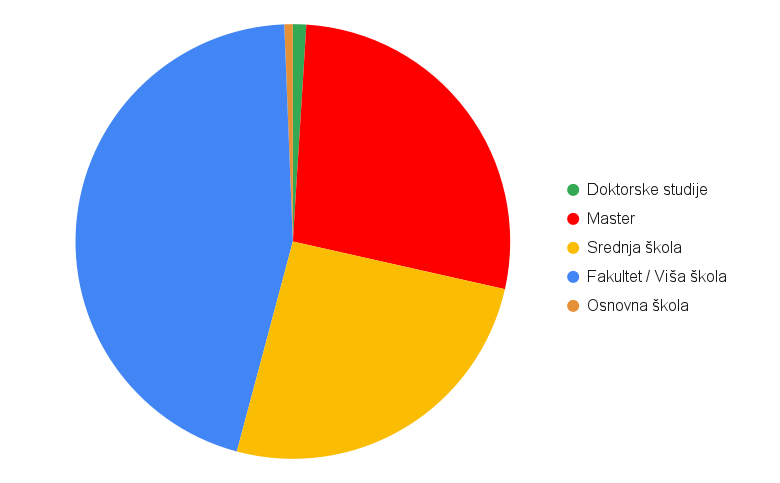
\includegraphics[scale=0.4]{PieChart.png}
\end{center}
\caption{Zaposleni u IT kompanijama po poslednje stečenom stepenu obrazovanja}
\label{fig:job-pie}
\end{figure}



Većina studenata koji se odluče da završe doktorske studije kao svoju glavnu motivaciju navode da bi želeli da jednog dana predaju na fakultetu ili da se bave naučno-istraživačkim radom. Ova činjenica može da objasni zašto je retko naići na doktore nauka koji rade isključivo u IT industriji.

\subsection{Veza akademske i industrijske zajednice}

Činjenica je da doktorat nije neophodan za rad u industriji, ali to ne umanjuje koliko su doktori nauka značajni za razvoj industrije. Naime, kompanije često sarađuju sa naučno-istraživačkim centrima i fakultetima u cilju razvoja novih tehnologija, optimizacije postojećih tehnologija i procesa u industriji. Mnoge kompanije osnivaju posebne grupe za istraživanje i razvoj (eng.~{\em R\&D - Research and Development}) i fakulteti ohrabruju i podržavaju priključenje doktoranata i profesora ovim projektima. Na primer, Katedra za računarstvo i informatiku Matematičkog fakulteta Univerziteta u Beogradu ističe da je otvorena za saradnju sa IT kompanijama u pružanju konsultativnih usluga u rešavanju problema kompanije, kao i za saradnju na naučno-istraživačkim projektima. Članovima Katedre je omogućeno da budu zaposleni pola radnog vremena na fakultetu, a pola u industriji na polju istraživanja i razvoja.\cite{katedra}

Istraživačko-razvojni institut za veštačku inteligenciju Srbije osnovan 2021. godine koji okuplja priznate srpske doktore nauka kao i mlade naučnike iz oblasti veštačke inteligencije aktivno sarađuje sa timovima iz \textit{Microsoft} Srbija i Elektroprivredom Srbije na poboljšanju predviđanja potrošnje električne energije. Ciljevi ove saradnje su između ostalog minimizacija troškova i umanjenje nepotrebnog angažovanja rezervnih proizvodnih kapaciteta.\cite{ivi} Isti institut takođe razvija inovativne tehnologije u automobilskoj industriji, konkretno, sisteme i senzore za automatsku vožnju zajedno sa kompanijom \textit{Contitental Automotive Serbia}\cite{continental}.

Razvojni centar kompanije Schneider Electric sa sedištem u Novom Sadu okuplja preko 30 doktora nauka iz oblasti energetike i računarstva. Cilj ove kompanije je razvoj tehnologija i rešenja za upravljanje energijom i procesima na bezbedan, pouzdan, efikasan i održiv način\cite{schneider}.

Domaći studio za razvoj video igara, \textit{Two Desperados}, osnovao je nezavisnu naučnu grupu za istraživanje i razvoj veštačke inteligencije za primenu u industriji video igara. U ovom timu, pored doktora matematike čija je uža stručna oblast algebra, rade i doktori informatike\cite{twoDesp}.

Grupa za programske jezike i alate (PLATO - \textbf{P}rogram \textbf{L}anguages \textbf{A}nd \textbf{TO}ols) Matematičkog fakulteta Univerziteta u Beogradu u naučno stručnoj saradnji sa istraživačko-razvojnim centrom \textit{Oracle Labs} aktivno radi na optimizaciji i unapređivanju kompajlerske infrastrukture \textit{GraalVM}. Neki od projekata podrazumevaju primenu mašinskog učenja u okviru \textit{GraalVM}-a, primena i efekti statičke analize u kompajleru i pisanje interpretera koji omogućavaju transparentni i efikasni poliglotizam između različitih programskih jezika\cite{plato}.

Saradnja na istraživačkim projektima i pružanje konsultativnih usluga IT kompanijama je značajna kako za same kompanije, tako i za akademsku zajednicu. Kroz saradnju sa visoko kvalifikovanim stručnjacima kompanije napreduju zahvaljujući razvoju inovativnih i optimizaciji postojećih tehnologija. Sa druge strane, studenti na doktorskim studijama i profesori stečeno znanje iz saradnje sa industrijom mogu da iskoriste u unapređenju i modernizaciji nastave na fakultetima.


\section{Zaključak}
\label{sec:zakljucak}

Sumiranjem dostupnih informacija o doktorskim studijama informatike u Srbiji, čitaocu su približeni uslovi upisa, tok studija kao i mogućnosti za vreme i nakon studija. Postoji mišljenje da su doktorske studije korisne samo za one koji bi želeli da ostanu da drže nastavu na fakultetu, ali jasno je uočena sve veća potreba za doktorima informatike u IT industriji koja se sve brže razvija. S obzirom na to da rad na fakultetu i u industriji nije međusobno isključiv, studenti doktorskih studija i doktoranti imaju priliku da se susreću sa interesantnim i izazovnim projektima koji bi doprineli daljem razvoju industrije.
Ostaje, međutim, problem ažurnosti i nedostatka relevantnih informacija koje bi čitaocima dale širu sliku, a možda čak i zainteresovale za doktorske studije informatike u Srbiji.


\addcontentsline{toc}{section}{Literatura}
\appendix
\bibliography{seminarski} 
\bibliographystyle{plain}


\end{document}
